\sys provides compiler support for \emph{automatic task generation} that simplifies programming writing task-based code by automatically translating C code into a task-based executable.  Translating C code into task-based code automatically requires identifying program points to use as task boundaries, defining a set of task functions that begin and end at those boundaries, ensuring that all existing control-flow paths are either contained within a task, or are made explicit in inter-task control-flow, and identifying and instrumenting accesses to task-shared variables that need to be protected by \sys at runtime.  The \sys compiler first analyzes the control-flow graph (CFG) and, using a rule-based heuristic, determines at which points to place a task boundary.  After identifying where to put task boundaries, the \sys compiler transforms the imperative code into tasks, instrumenting protected memory accesses. 

%The compiler consists of two {\em passes} that runs on LLVM Intermediate Representation (IR)\todo{Which version?}{Kiwan}---an intermediate language generated by Clang~\cite{clang_website}:
%
%\begin{enumerate}
%	\item \textbf{Analysis Pass}, which analyzes the code structure and decides where to put task boundaries;
%	\item \textbf{Transform Pass}, which converts the code into task-style program and fills it with necessary \sys keywords so that it can run on \sys.
%\end{enumerate}
%
%We shall now proceed with describing these two parts in detail.

\subsection{Task Boundary Identification Analysis}
\label{sec:compiler_analysis_pass}

\todo{Define single entry}{Kiwan}
\TODO{Brandon: the term "single-entry" is well-known in the community to mean that there is a single control-flow edge entering the task. Thinking about this a bit, is there a simple reason why we cannot have multiple-entry tasks? A totally plausible task graph could be like A->B B->C C->B C->A; here, B has two predecessors.  Is this fundamental?  Or an analysis convenience? I've left it as "single-entry" for now}

\sys analyzes a program to determine where to put task boundaries to divide the
program into tasks. A task is a single-entry, multiple-exit region of the CFG
and in a correct task decomposition, no task should ever consume more energy
than the device's energy buffer can store.  There are several factors that
determine whether tasks will execute efficiently. A task decomposition should
minimize the number of variables that are accessed by multiple tasks and, 
consequently, must be protected by \sys's paging mechanism.  Tasks should
be roughly the same size, simplifying \sys's dynamic reasoning about coalescing
by eliminating the need to consider variable task cost at run time.  To minimize
overhead introduced at task boundaries (i.e., commit), a task decomposition should 
maximize task size, which minimizes the frequency of task transitions.


%\begin{enumerate}[label={\bf C\arabic*:}]
%\item{No task should ever use up more energy than what the capacitor of the system can provide;} \TODO{We do not (cannot, actually) guarantee this, so I think we can, at best, say that this is an optimization constraint.  What do you think?}
%\item{A task should be single-entry.}\todo{Define single entry}{Kiwan} 
%\end{enumerate}
%
%For a task-decomposition to be efficient, the compiler should optimize the following points:
%
%\begin{enumerate}[label={\bf O\arabic*:}]
%\item{Tasks should be roughly the same size for efficient coalescing;}
%\item{The number of protected variables should be minimized;}
%\item{Task boundary should be visited as least as possible due to overhead on boundaries.}\todo{Define overhead on boundaries}{Kiwan}
%\end{enumerate} 

\sys meets these correctness and efficiency requirements with a four-part
analysis composed of (i) \emph{graph construction}, (ii) \emph{loop analysis},
(iii) \emph{task preparation}, and (iv) \emph{single entry assurance}.

\begin{figure}
	\centering
	\subfloat[Plain C code]{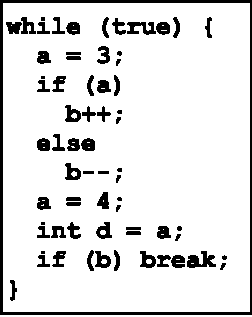
\includegraphics[width=0.3\columnwidth]{figures/compiler1.pdf}\label{fig:comp_1}}
	\subfloat[Boundary placement]{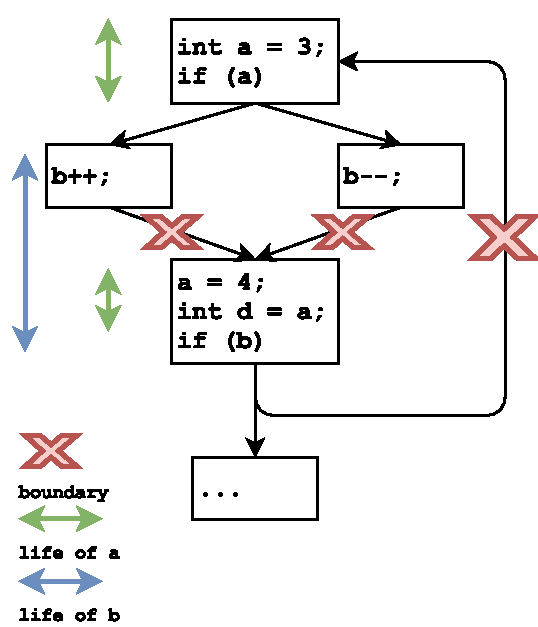
\includegraphics[width=0.3\columnwidth]{figures/compiler2.pdf}\label{fig:comp_2}}
	\subfloat[Code Transformation]{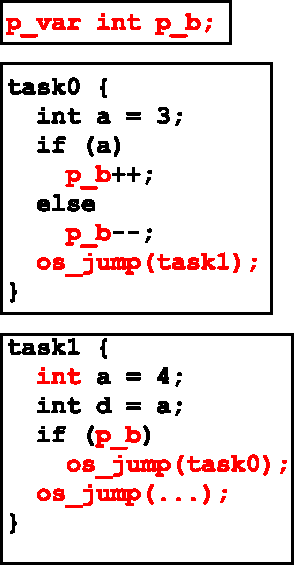
\includegraphics[width=0.3\columnwidth]{figures/compiler3.pdf}\label{fig:comp_3}}
	\caption{Illustration of \sys compiler task division operation.\todo{Make figures of the same readable size}{Przemek}}
	\label{fig:compiler_overview}
\end{figure}

\textbf{Graph Construction:} starting from a plain C code (see example in Figure~\ref{fig:comp_1}) \sys compiler first builds a control flow graph where (i) each vertices is a \emph{basic block} and (ii) each unidirectional edge is a \emph{branch from one basic block to another} (see example in Figure~\ref{fig:comp_2}). All function calls are inlined in the main function prior to building a graph.

Each vertex has a {\em cost}, which represents the energy usage of the basic block. We used the number of LLVM IRs inside a vertex as the energy use metric. When forming a task, each task should contain a basic block so that the sum of cost of all blocks within each tasks should be roughly the same (viz. O1) and does not exceed given energy budget (viz. C1). For our implementation, the programmer should provide the energy budget in compile time defined in number of LLVM IR instructions that the hardware can execute safely in one energy cycle. This number must be found experimentally.

Each edge holds the information about the {\em live variables} across the edge, and if the edge is within any loop, the {\em loop count}. By this information, the compiler tries to minimize the number of protected variable (viz. O2), because placing boundary at an edge means the live variables across that edge need to be protected. Also the compiler avoids placing boundaries at an edge that is within a loop whose loop count is big (viz. O3).

The compiler also calculates a dominance relation \todo{Define dominance relation}{Kiwan} between vertices. This information is used to ensure task's single-entry property (viz. C2).

\textbf{Loop Analysis:} After constructing the graph and assigning the information on a cost and live variables to each vertex and edge, respectively, the compiler begins with analyzing the program loops. The compiler first identifies all loops and then multiplies the loop count by the cost of a vertices within the loop. The reason is, if the loop is inside a task it will use up energy that is roughly multiplied by the loop count compared to code that is outside of a loop. If the resulting cost of a loop is too large\todo{how do you decide on the acceptable loop cost?}{Kiwan}, the compiler places boundary at the back edge of the loop, and reverts the change to the cost of the vertices inside. It means that if the loop is too large to fit in one task, each iteration should be a separate task execution.

If a program has an unbounded loop (such as {\tt while} statement), the compiler conservatively assumes the loop count to be very large. The programmer can prevent this by annotating maximum possible loop count of such unbounded loop if the programmer has the information.\todo{'the' or 'this'? Does it mean programmed still needs to inspect the code?}{Kiwan}

\textbf{Tasks Preparation:} After initial boundary placemen with loops analysis, the compiler places additional boundaries if some tasks are still too large. The \sys compiler starts from the beginning of the main function and traverse through the graph in a depth-first search manner. If any part of the graph is found that is too long to fit in the energy bound, it means a boundary must be placed somewhere within. The subset of graph that needs boundary placement within is called a {\em boundary-candidate}.

As discussed above, when placing boundary we take three optimization criteria into account: \{O1, O2, O3\}. We now introduce a heuristic that consider all these criteria and choose the local optimum\todo{Optimum of what?}{Kiwan}. The heuristic calculates the {\em score}, $S$, of each edge inside the boundary candidate as
%
\begin{equation}
S = \frac{w_{0} N_{\text{IR}} - w_{1} N_{\text{PV}}}{N_{\text{loop}}},\nonumber
\end{equation}
%
where $N_{\text{IR}}$ is a normalized IR count that the task will end up having if the compiler places boundary at the specific edge, $N_{\text{PV}}$ is the number of protected variables that will be newly introduced by placing boundary at the edge, and choose the edge with the highest score, $N_{\text{loop}}$ is the loop count and $w_{0},w_{1}\in [0,1]$ are pre-selected weights before compilation\footnote{Naturally, different $w_{0}, w_{1}$ will have different effect on the compiler result. We will study this effect in Section~\ref{sec:results_compiler}.}. Both $N_{\text{IR}}$ and $N_{\text{PV}}$ are normalized within the boundary candidate, since usually IR count is much larger and has higher variance, thus has dominating effect if not normalized. It is better to have higher IR count within the task since it means the task size is similar to the size given by the programmer (viz. C1). On the other hand, change in protected variable is better to be small (viz. C2), so we penalize it by assigning a negative value to $N_{\text{PV}}$. If the edge is within a loop, the score is divided by $N_{\text{loop}}$. It will result in not placing boundary within loops unless other parts of the formula really pays off (viz. C3)\todo{This sentence is not clear: what "pays off" means in this context?}{Kiwan}. Note that complier never makes a decision that will end up in having more IR count than the programmer specified because at the beginning boundary candidate is chosen to have less IR than the programmer specified number.

Figure~\ref{fig:comp_2} shows example of such boundary placement on graph. The first three vertices will become one task while the rest will become another (see Figure~\ref{fig:comp_3}).

\textbf{Ensuring Single Entry:} After placing a boundary, the compiler ensures that the newly made task is single-entried by checking dominance relation. That is, every vertex within a task should be dominated by the entry vertex of the task. If this rule is violated, the compiler places additional boundaries to make sure that every task is single entried.

\subsection{Compiler Transform Pass}
\label{sec:compiler_transform_pass}

In the compiler transform pass, a complier executes sub-tasks described below.

\textbf{Declaring and Migrating Codes to Tasks:} After the boundary placement is finished, the analysis pass passes the information to transform pass. The transform pass makes new task, traverse through the graph, and copies every code within the vertices it encounters to the new task until it meets the task boundary. At the task boundary, it makes another task and starts copying again, and repeat this action until every code is moved to form a task.

\textbf{Renaming Variables:} On copying the code, the variables should be renamed. If a variable is alive across multiple tasks, it needs to become a global-protected variable, and every access to the variable should be redirected. If a variable's live range is local to the task, it does not need to go through such renaming. For example, in Figure~\ref{fig:comp_2}, boundary is placed within the live range of variable {\tt b} (Note that the red cross overlaps the blue arrow). Thus variable {\tt b} needs to become a protected variable {\tt p\_b} and every access to {\tt b} should be redirected to {\tt p\_b} (Figure~\ref{fig:comp_3}). On the other hand, {\tt a}'s live range is always local to a single task. In such case, it need not become a protected variable. Note, however, still new declaration of {\tt a} should be inserted in {\tt task1} (Figure~\ref{fig:comp_3}). As an improvement to the complier, constants and read-only variable never becomes protected.

\textbf{Inserting \texttt{os\_jump} Calls:} After renaming is done, the compiler detects the broken {\tt branch} instructions\todo{Define protected branch instruction}{Kiwan} which tries to branch to a basic block that is inside different task and change it to an {\tt os\_jump} call (Figure~\ref{fig:comp_3}).  Note that in this figure we showed the name of the next task to be executed for readability, however {\tt os\_jump} call takes offset number as an argument. In reality the compiler statically calculates and passes the offset.

\textbf{Dealing With PHI Nodes:} Whenever more than two different control flows try to write different value in the same memory location, LLVM makes a unique IR called {\em PHI Node} when reading the memory location~\cite{}. However if there is a boundary between the memory write and the PHI Node, the compiler will not work. Thus, on each of this occurrence, \sys compiler declares a special protected variable and makes the write relocated to the protected variable. Then the PHI Node becomes simply a read to a protected variable.

\textbf{Inserting API Call for Paging:} To run \sys, every read or write to a protected variable should call related API for page swapping and dirty page marking. The compiler conservatively inserts such calls before a {\em possible} read or write to the protected variable. We use the basic pointer alias feature provided by the LLVM library. We are being conservative, so it is always correct, albeit not always efficient.\todo{We need to say more about the level of this inefficiency and how it is measured}{Kiwan}

\textbf{Creating New Main Function and Cleaning Unnecessary Codes:} After task generation is done, the compiler generates new main function and peppers the system with necessary codes that is needed by \sys (such as code for evoking {\tt os\_sceduler}). Also it removes the code that became stale (such as the body of a function call, for all the function calls are now inlined).

\subsection{Compiler Design Decisions}
\label{sec:compiler_limitations}

To be able to implement \sys compiler certain critical assumptions had to be made. 

\begin{enumerate}
	%
	\item \textbf{Conservative handling of unbounded code sections:} When a C program contains an unbounded loop, the \sys compiler makes a conservative decision of regarding its loop count to be very large. However, if a programmer annotates the expected loop count manually the overhead can be relieved.
	%
	\item \textbf{Conservative handling of pointers:} When a C program contains pointer, due to the limitation of pointer alias, the compiler makes the conservative decision. That is, it may consider a variable's live range longer than actual, or it may insert API call for page swap even when it is unnecessary. However, these overhead can be reduced by better pointer aliasing algorithm.
	%
	\item \textbf{Function call inlining:} \sys compiler inlines all function call prior to analysis for simplicity. However it can introduce code bloat. Insted, a better way would be to convert large-frequently visited functions to a separate task and make the function call a jump to the task. However we did not implemented such feature for simplicity of the system.
	%
	\item \textbf{LLVM IR instruction count to estimate the energy usage:} The compiler uses the number of LLVM IR count as an indicator for energy usage in trying to meet correctness constraint C1 and optimization constraint O1. Intuitively, the number of LLVM IR correlates with the energy usage since more instructions will lead to more energy usage. However, we need to be aware that is nevertheless a crude approach of estimating energy consumption---actual machine instructions are what counts and they are not exactly equal to the LLVM IR. Also, different instructions have different power usage, and even same instruction has different energy usage from time to time (for example cache hit and miss makes even the same {\tt load} instruction to use different amount of energy). However, the energy usage of each task need not be exactly the same to what programmer indicated, and it is sufficient to make sure that all of the tasks are small enough to fit in to the energy budget. Therefore we conjecture that from the \emph{implementation simplicity perspective} of \sys's compiler counting the LLVM IR instruction is sufficient. The programmer can always ensure correctness constraint C1 by conservatively providing IR count in compile time that is empirically proven to be safe. Also, since the estimation of energy usage of each basic block is perpendicular to the compiler itself, it is simple to plug in a better energy model if there is one.
	%
	\item \textbf{Limitation of the boundary placement heuristics:} The boundary placement strategy is a heuristic that chooses the local optimum. However, selecting every local optimum might not be the global optimal solution. We can instead do a random search multiple times to find a global optima. Since current heuristic is already showing good result that is comparable to human-written code, refer to Section~\ref{sec:results_coalescing}, we leave such optimization as a future work.
\end{enumerate}
